\documentclass[border=6pt]{standalone}
\usepackage{tikz}
\usepackage[edges]{forest}
\usetikzlibrary{arrows.meta,positioning,calc,decorations.pathreplacing,shapes.geometric}
\begin{document}
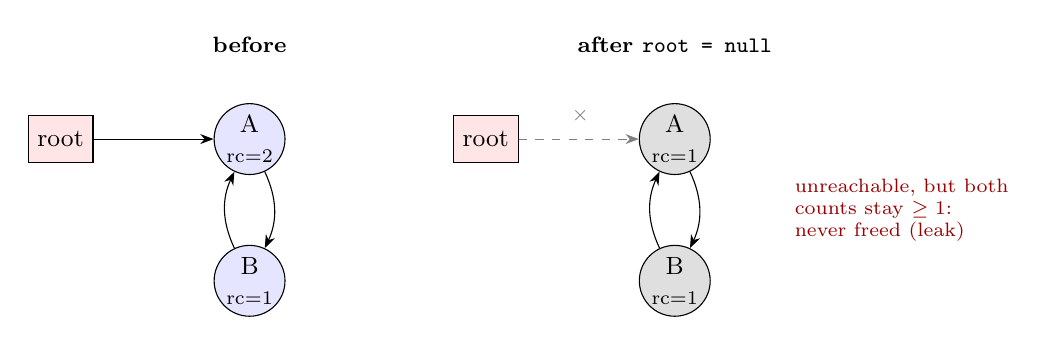
\begin{tikzpicture}[>=Stealth,font=\small,
 v/.style={draw,circle,minimum size=0.9cm,inner sep=0pt,align=center}]
\node[font=\footnotesize\bfseries] at (1.2,2.2) {before};
\node[draw,rectangle,fill=red!10,minimum size=0.6cm] (r) at (-1.2,1.0) {root};
\node[v,fill=blue!10] (a) at (1.2,1.0) {A\\{\scriptsize rc=2}};
\node[v,fill=blue!10] (b) at (1.2,-0.8) {B\\{\scriptsize rc=1}};
\draw[->] (r)--(a); \draw[->] (a) to[bend left=25] (b); \draw[->] (b) to[bend left=25] (a);
\node[font=\footnotesize\bfseries] at (6.6,2.2) {after \texttt{root = null}};
\node[draw,rectangle,fill=red!10,minimum size=0.6cm] (r2) at (4.2,1.0) {root};
\node[v,fill=gray!25] (a2) at (6.6,1.0) {A\\{\scriptsize rc=1}};
\node[v,fill=gray!25] (b2) at (6.6,-0.8) {B\\{\scriptsize rc=1}};
\draw[->,dashed,gray] (r2)--(a2); \node[font=\scriptsize,gray] at (5.4,1.3) {$\times$};
\draw[->] (a2) to[bend left=25] (b2); \draw[->] (b2) to[bend left=25] (a2);
\node[font=\scriptsize,anchor=west,red!60!black,align=left] at (8.0,0.1) {unreachable, but both\\counts stay $\ge 1$:\\never freed (leak)};
\end{tikzpicture}
\end{document}
